\documentclass[AER]{AEA}
\usepackage{amsmath}
\usepackage{graphicx}
\usepackage{harvard}
\usepackage{hyperref}

\begin{document}

\title{Temporal Fusion Transformer Models for Predicting Stock Behavior}
\shortTitle{TFT Stock Behavior Prediction}
\author{Andrew Lys\thanks{Lys: University of Chicago, andrewlys@uchicago.edu}}
\date{\today}
\pubMonth{3}
\pubYear{2025}
\JEL{}
\Keywords{}

\begin{abstract}
Your abstract here.
\end{abstract}


\maketitle
In portfolio design, a very common, and profitable strategy is called quantitative value investing. 
This strategy consists of designing some objective measure, ranking stocks based on this measure, and investing into the top ranked 
companies. The measure is derived from expert knowledge about how markets function, data, or some combination 
of the two. Portfolio design, in general, has been a field slow to adopt machine learning techniques, generally 
forgoing the data driven aspect of constructing these measures in exchange for more traditional financial 
measures. Examples of these measures include Trailing Twelve Month Returns (TTM Returns) and Earnings Before 
Interest and Taxes/Enterprise Value (EBIT/EV). These measures are often called value factors, as in the 
Fama-French value factor model. A clear drawback of this method is that there are countless different value 
factors an analyst could choose. For instance, what if it's  the case that ranking stocks based on Trailing 
Eighteen Month Returns, instead of TTMs, is the secret to beating the market? Of course this example is silly, 
but in this manner, in their use as feature engineers, Neural Networks serve as an obvious next step to improve 
this strategy.

In traditional computer vision learning techniques, like boosted decision trees for facial recognition 
\cite{ada-boost}, the main hurdle was always the development of better methods to extract relevant features. 
With the advent of convolutional neural networks, able to extract relevant features automatically, computer 
vision was effectively revolutionized \cite{alexnet}. Why can't Neural Networks do the same for factor 
engineering? Humans are bias-prone. When we pick factors, we are unintentionally choosing factors that are not 
statistically clean. Analysts have subconscious reasons for selecting factors, no matter how hard they can try 
to avoid these biases. For instance, if an analyst truly believes in a company, they might unintentionally 
choose factors that bias them towards that company, but will ultimately lead to lower returns overall. For 
reasons like this, Neural Networks have the capacity to revolutionize forecasting in the same way as they did 
image recognition. 

Financial fundamental data is in the form of time series data, and thus admits a very natural sequence 
structure that can be leveraged by Recurrent Neural Networks (RNNs). \cite{euclidean} investigated the use of 
Long Short Term Memory (LSTM) RNNS in forecasting fundamental data. These are RNN architectures where there are 
two streams of data passing through the recurrent neural network, the long term and short term streams. In this 
paper, we will investigate the use of Temporal Fusion Transformers (TFTs), as proposed by \cite{tft}. We use 
the implementation provided by PyTorch Forecasting. TFTs are a novel architecture developed by Google in collaboration with the University of Oxford. 
They leverage the recent success of Transformers in natural language processing, and the natural sequence
structure of time series data. \cite{tft} found promising results in forecasting, so we will investigate their
ability to predict stock behavior.

So far, we have been careful to avoid forecasting. This is because forecasting is very difficult. 
\cite{euclidean} found that there is far too much noise to be able to accurately generate forecasts that meaningfully 
outperform linear models. For this reason, we focus on a far more tractable problem. We will attempt to predict
certain qualitative features of stock behavior. The main feature we will focus on is whether a stock is a value trap.

In the quantitative value investing strategy, we seek to select stocks that are, in some sense, undervalued.
We approximate this true value of a stock by variuous value factors. 
The value factors we select maybe misleading, causing us to misunderstand the true value of a stock.
In this way, we may select stocks that are not actually undervalued, but are instead value traps.
A stock may perform very well on our value factors, but there may be some aspect we are missing in our analysis
that will cause the stock to perform poorly in the future. For instance, a stock may have a high EBIT/EV ratio,
but if the company is about to go bankrupt, this ratio will not be very useful. 

This problem is significantly more tractable than forecasting, and is in fact, very valuable. \cite{euclidean}
have shown that identifying value traps can result in a 3.5\% increase in annualized returns (See Figure \ref{fig:clairvoyant}).

\begin{figure}[ht] 
    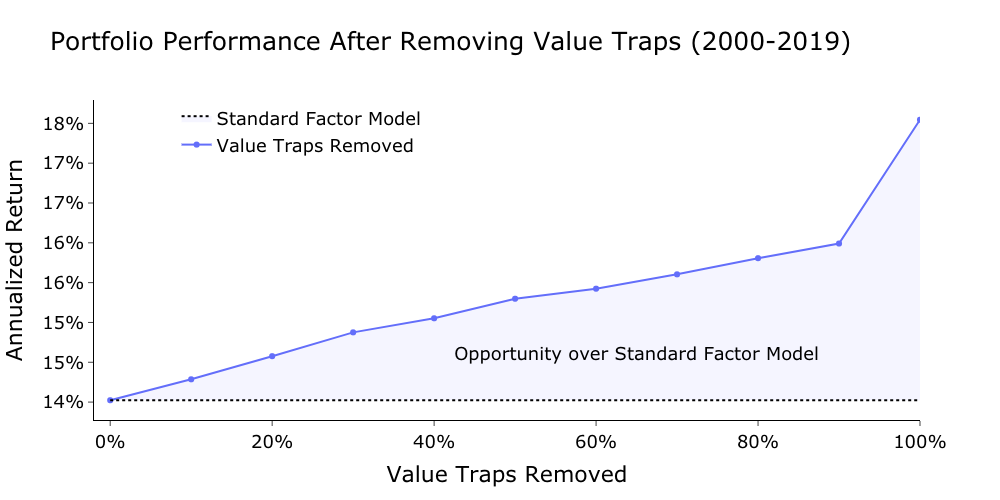
\includegraphics[scale = 0.3]{value_trap_clairvoyant_2.png}
    \caption{Portfolio performance as an increasing number of value traps are removed.}
    \label{fig:clairvoyant}
\end{figure}

In this paper, we will investigate the ability of TFTs to predict whether a stock is a value trap.
The structure of the paper is as follows: in section 2, we will discuss the data and the pre-processing; 
in section 3, we will discuss the model framework; In section 4, we will present the experimental setup
and the results; and in section 5, we will conclude.
\section{Data and Data Pre-Processing}
\subsection{Raw Data}
The data we use is from the Wharton Research Data Services (WRDS) database.
We use the Compustat North America database, which contains fundamental data on companies.
As undergraduate students, we are able to access this data through the University of Chicago's library,
although, without a PI, we are only able to get a day pass.

We focused on the time frame 1970-2025, since before 1970, fundamentals reporting was not as standardized.
Additionally, we only considered companies that are located in the United States. We filtered for companies
only traded on either the NYSE, NASDAQ, or AMEX. We also filtered out financial services companies. 
The motivation for this is that the fundamentals reporting of financial services companies represent
very different things than for industrial companies. Although this reasoning may be disputed, 
\href{https://alphaarchitect.com/why-exclude-financial-firms-from-quantitative-studies/}{this is considered
a common practice}. The data was taken in quarterly intervals, since this is how often companies report
fundamental data. This represents a total of approximately 12,000 companies, and a total of 876,347 observations.

Following \cite{euclidean}, we selected the following source fields, as show in Table \ref{tab:source_fields}.

\begin{table}[ht]
    \centering
    \begin{tabular}{|c|c|}
        \hline
        \textbf{Income Statement \& Other Items} & \textbf{Balance Sheet} \\
        \hline
        Sales (Revenue) & Cash \& Cash Equivalents \\
        Cost of Goods Sold & Receivables \\
        Sales, General, and Admin Expenses & Current Assets \\
        Operating Income After Depreciation & Property Plant \& Equipment \\
        Net-Income & Other Assets (Incl. Goodwill) \\
        Capital Expenditures & Total Assets \\
        Dividends & Debt in Current Liabilities \\
        Common Shares Outstanding & Accounts Payable \\
        Price per Share & Current Liabilities \\
        & Long-Term Debt \\
        & Other Liabilities \\
        & Total Liabilities \\
        & Minority Interest \\
        & Preferred Stock \\
        & Shareholders’ Equity \\
        \hline
    \end{tabular}
    \caption{Selected Source Fields}
    \label{tab:source_fields}
\end{table}
\subsection{Pre-Processing}
There is a lot of pre-preprocessing that needs to be done before we can use this data in a model. 
We cannot simply feed the raw data into the model. 
For each company, there are very unique patterns in the raw data that the model will memorize.
As a result, the model will not be able to learn. We need to apply some processing to the data to make sure
this does not happen. Additionally, there are some other financial features that we know we want to include.
Since this data is fairly noisy, there are some NaNs that we need to deal with. 
We will develop a NaN policy for dealing with missing data.
Finally, following the reccommendation of \cite{seasonalization}, we will apply a seasonalization algorithm to these features.
We will then feed the original features in alongside the seasonalized features.
Additionally, we will need to apply some sort of normalization to the data before the seasonalization. 
These two will be discussed in the next section.

We will end up with five categories of features: 
\begin{itemize}
    \item Momentum Features
    \item Valuation Features
    \item Fundamental Features
    \item Missing Value Features
    \item Seasonal Features
\end{itemize}
\subsubsection{Momentum Features}
Since it's quite likely that recent stock price changes will be indicative of future stock price changes,
we will include some momentum features, in order to make it easier for the Neural Network to find these patterns.
We will include 3, 9, 12, and 18 month percent changes in stock price.
Additionally, we will provide the percentile rankings amongst stocks traded during that quarter of these features.
These features will hopefully allow the Neural Network to find these patterns easier, and make use of them.
\subsubsection{Valuation Features}
We will include the following valuation features: Book to Market and Earnings Yield.
These are common value factors used in the Fama-French model.
They are defined as follows:
\begin{itemize}
    \item 
        bkmktq: Book to Market
        $$\text{Book to Market } = \frac{\text{Shareholder Equity}}{\text{Closing Price } \cdot \text{ Common Shares Outstanding}} $$
    \item
        evq: Enterprise Value
        \begin{align*}
        \text{Enterprise Value} &= \text{Closing Price } \cdot \text{ Common Shares Outstanding}\\
        &+ \text{ Long Term Debt } + \text{ Debt in Current Liabilities}\\
        &- \text{ Cash and Short Term Investments}
        \end{align*}
    \item
        eyq: Earnings Yield
        $$
        \text{Earnings Yield} = \frac{\text{Operating Income After Depreciation}}{\text{Enterprise Value}}
        $$
\end{itemize}
Additionally, we provide percentile rankings alongside these features.
\subsubsection{Fundamental Features}
We include all of the fundamental features we selected in Table \ref{tab:source_fields}, but we first have to transform them.
\subsubsection{NaN Policy}
We follow the NaN policy given by \cite{nanpolicy}. For each feature, we add an additional NaN indicator feature that is 1 if the feature is NaN, and 0 otherwise.
We then fill the NaNs with the previous value. If there is no previous value, we fill it with 0.
We obviously, do not normalize these features.
The advantage of this policy is that as opposed to mean imputation or some other form of imputation is that it 
allows the Neural Network to learn why data is missing. For instance, if a company is missing financial reports,
that's a pretty good indicator that company is in trouble. Providing the Neural Network with these features
will hopefully let it learn these patterns.
\subsection{Transformation and Deseasonalization}
For the transformation, we follow the reccommendation given by \cite{meanscale} and apply a meanscale transformation, followed by a log-scale transformation.
However, before we do this, \cite{meanscale} assumes that all the data is strictly positive. 
This is not the case for our data, but we can simply add a constant to all the data to make it positive.
This will not change any of the predictions on the data, but will allow us to apply the log-scale transformation.
To summarize, if $C$ is the minimum value in our entire data set, we first shift all the data by $|C|$. 
Letting $X_{i}$ be a company, and $X_{i,t}$ be the vector of features at time $t$, we apply the following transformation:
\[
X_{i,t} \mapsto X_{i,t} + |C|
\]
Now, we apply the meanscale transformation:
\[
X_{i,t} \mapsto \frac{X_{i,t}}{1 + \frac{1}{t}\sum_{s=1}^{t} X_{i,s}}
\]
Finally, we apply the log-scale transformation:
\[
X_{i,t} \mapsto \log(X_{i,t} + 1)
\]
We do not apply the transformation to the NaN indicator features, nor the percentile ranking features.
We apply the transformation to the momentum, valuation, and fundamental features.

We then apply a seasonalization algorithm to the transformed features, to obtain seasonal features. 
I.e. we apply the following transformation:
\[
X_i = \hat{S}_i + \hat{T}_i + \hat{R}_i
\]
Where $\hat{S}_i$ is the seasonal component, $\hat{T}_i$ is the trend component, and $\hat{R}_i$ is the residual component.
We feed $\hat{S}_i$ into the model, alongside the original features.
We use the python implementation of STL provided by statsmodels.
We apply the seasonalization to the momentum, valuation, and fundamental features. 
We do indeed apply the seasonalization to the percentile ranking features, since there might be seasonality in the rankings.
We apply the seasonalization because we believe that the deseasonalized trends will be a helpful feature for the Neural Network to learn.

In total we will end up with approximately 130 features.
\section{Model Framework}
We use the Temporal Fusion Transformer (TFT) model, as proposed by \cite{tft}. 
We use a fixed window size of 5 years, or 20 quarters. We output 20 quarters into the future. 
We additionally add an extra year gap between the input and output in order to avoid seasonal effects.
We split our data into a training set, a validation set for hyperparameter tuning, and a test set.
The split is as follows:
\begin{enumerate}
    \item Training set: 1970-2001,12,31
    \item Validation set: 2002,1,1-2009,12,31
    \item Test set: 2010,1,1-2025,12,31
\end{enumerate}
We use the PyTorch Forecasting library to implement the model.
We fix the the number of LSTM layers to 2 and the loss function is the logistic loss function.
We optimize the following hyperparameters:
\begin{itemize}
    \item Hidden Size
    \item Attention Head Size
    \item Hidden Continuous Size
    \item Learning Rate
    \item Reduction On Plateau Patience
    \item Gradient Clip Value
    \item Dropout Rate
\end{itemize}
\section{Experimental Results}
\section{Conclusions}
One of the main issues with this model is that we face a remarkable lack of data.
Despite the fact that we have nearly a million observations, this number is not actually how many samples we get to train on.
A single observation is actually a contiguous 5 year time series for a single company. 
This reduces the number of training samples to around 57,320, which is barely enough to train a deep neural network.
The total number of actual parameters in our model is about 259,000. 
Although it is very common to train models with far more parameters than samples, the lack of data is still a major issue.
One interesting way to address this is to use a generative model combined with transfer learning.
We could train a generative model to generate synthetic data and then use this synthetic data to train a model, which we further finetune with our real data.
The motivation is that we have certain expert knowledge about how markets should function, and we can use this to generate synthetic data.
Of course the synthetic data will be mostly trash, but it will still force the model to learn something about the data.
This approach has been explored by \cite{dataAug} with impressive results on LSTMs. 
They did not test this approach on the TFT model, which generally performs better than LSTM models in forecasting tasks.
This is a very interesting direction for future research.

Another limitation of this model is not just the lack of data, but the lack of features. 
Fundamentals data is fantastic for forecasting, but it is not enough. 
There are many other features that would help capture the true value of a stock.
One interesting feature that could be added is the sentiment of the market. 
There have been many studies that explore deep learning for natural language processing of financial news.
\cite{sentimentAnalysis} is a good survey of the literature.
Adding these features could be the step needed to identify all the value traps. 
In fact, this might help make forecasting more tractable, as the sentiment of the market is a very important feature in forecasting.

Despite this, we see that the TFT model is able to predict value traps with a high degree of accuracy. 
It does better than the LSTM model presented by \cite{euclidean}. 
\bibliographystyle{aea}
\bibliography{references}

% The appendix command is issued once, prior to all appendices, if any.

\end{document}

